%----------------------------------------------------------------------------------------
%	PACKAGES AND OTHER DOCUMENT CONFIGURATIONS
%----------------------------------------------------------------------------------------

\documentclass[
	12pt, % Default font size, values between 10pt-12pt are allowed
	%letterpaper, % Uncomment for US letter paper size
	%spanish, % Uncomment for Spanish
]{fphw}

% Template-specific packages
\usepackage[utf8]{inputenc} % Required for inputting international characters
\usepackage[T1]{fontenc} % Output font encoding for international characters
\usepackage{mathpazo} % Use the Palatino font

\usepackage{graphicx} % Required for including images

\usepackage{booktabs} % Required for better horizontal rules in tables

\usepackage{listings} % Required for insertion of code

\usepackage{enumerate} % To modify the enumerate environment

%----------------------------------------------------------------------------------------
%	ASSIGNMENT INFORMATION
%----------------------------------------------------------------------------------------

\title{Devoir Maison} % Assignment title

\author{Durand Enzo 21107517} % Student name

\date{November 24th, 2021} % Due date

\institute{Sorbonne Université} % Institute or school name

\class{Algorithmes sur les arbres et les graphes en bio-informatique (AAGB)} % Course or class name

%\professor{Dr. Albert Einstein} % Professor or teacher in charge of the assignment

%----------------------------------------------------------------------------------------

\begin{document}

\maketitle % Output the assignment title, created automatically using the information in the custom commands above

%----------------------------------------------------------------------------------------
%	ASSIGNMENT CONTENT
%----------------------------------------------------------------------------------------

\section*{Exercice 1}

\begin{problem}
	1. Qu'est ce qu'une matrice de coût ? Quelles données pour la construire ? Comment la construire ? Donner un exemple.
\end{problem}
\begin{center}
	\begin{itemize}
		\item Une matrice de coût est une matrice qui contient les valeurs associées aux match/mismatch pour chaque lettre de l'alphabet étudié. Les indices de ligne et de colonne correspondent aux deux séquences étudiées.
		\item Pour construire une matrice de coût, on a donc besoin des différentes lettres contenues dans les séquences que l'on compare ainsi que des valeurs de match/mismatch associées aux lettres de l'alphabet.
		\item Pour exemple, on a la matrice blossum qui permet d'avoir les valeurs de match et mismatch pour un alphabet correspondant à des acides aminés: 
			\begin{center}
				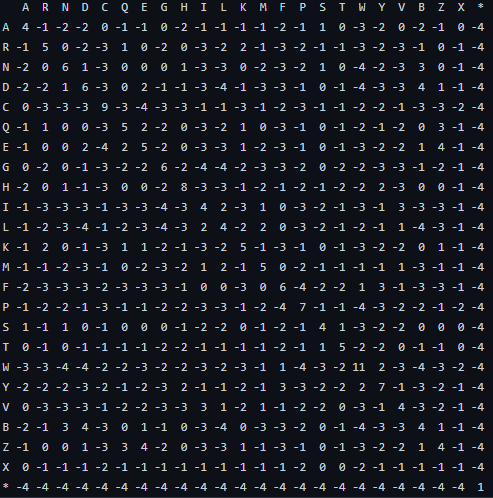
\includegraphics[width=0.5\columnwidth]{blossum.png} % Example image
			\end{center}
	\end{itemize}
\end{center}

\begin{problem}
	2. Comment comparer deux séquences ? Quelle est l'utilité de la matrice de coût pour cela ? Citer deux méthodes vues en TD pour comparer deux séquences.
\end{problem}
\begin{center}
	\begin{itemize}
		\item Pour comparer deux séquences, il faut trouver l'alignement global ou les alignements locaux de son alphabet. On les trouve en donnant des valeurs positives à des lettres qui concordent et en donnant une pénalité aux lettres qui ne concordent pas. Lorsque l'on a pas de matrice de coût, on donne la même valeur positive et la même valeur de pénalité à toutes les lettres suivant les match/mismatch.
		\item La matrice de coût permet de donner une pénalité différente suivant la différence des lettres dans la séquence. En effet, il est parfois judicieux de punir plus fortement une différence d'acide aminé polaire/apolaire comparé à une différence d'acide aminé du même groupe.
		\item Les deux méthodes que nous avons étudié en TD sont le Dot Plot et l'algorithme de Needleman \& Wunsch.
	\end{itemize}
\end{center}

\begin{problem}
	3. Définisser orthologie, paralogie, analogie et homologie. Pourquoi chercher des homologies entre séquences ?
\end{problem}
\begin{center}
	\begin{itemize}
		\item L'orthologie est le lien évolutif entre deux gènes présents chez deux espèces différentes. On dit de deux séquences qu'elles sont orthologues si elles descendent d'une séquence unique présente chez leur dernier ancêtre commun. Le gène impliqué résulte d'une spéciation.
		\item La paralogie est le lien évolutif entre deux gènes présents chez deux espèces différentes. On dit de deux séquences qu'elles sont paralogue si elles descendent d'une séquence unique présente chez leur dernier ancêtre commun mais contrairement à l'othologie, le gène impliqué résulte d'une duplication suivie d'une spéciation. Ce gène peut donc avoir de nouvelles fonctions.
		\item L'analogie est une similitude entre deux expressions du phénotype qui ont les mêmes fonctions biologiques chez deux espèces différentes. Ces deux expressions phénotypiques ne proviennent pas d'une descendance avec un ancêtre commun. Le gène est donc apparu une fois sur chacun des ancêtres communs des deux espèces.
		\item L'homologie est un lien évolutif entre expressions phénotypiques de deux espèces différentes, provenant d'une descendance avec un ancêtre commun.
		\item Il faut chercher les homologies pour pouvoir construire des arbres phylogénétiques afin de mieux comprendre l'évolution de certaines espèces. On peut faire cela avec des algorithmes comme UPGMA ou NJ.
	\end{itemize}
\end{center}

%------------------------------------------------

\section*{Exercice 2}

\begin{problem}
	1. Définissez l'horlogie moléculaire et expliquer pourquoi on emploie ce terme pour l'algorithme UPGMA.
\end{problem}
\begin{center}
	\begin{itemize}
		\item L'horloge moléculaire est une hypothèse en biologie selon laquelle les mutations du génome se feraient à vitesse constante. Grâce à cette hypothèse, on peut donc mettre en corrélation le taux de mutation et les divergences génétiques de différentes espèces afin de trouver une chronologie d'apparition des espèces.
		\item On emploie ce terme pour UPGMA car cet algorithme construit un arbre phylogénétique à partir d'une matrice de distance. Il donne des tailles de branches équivalentes aux différentes espèces proportionnellement à leurs écarts de nucléotides. Il construit donc cet arbre en se basant sur l'hypothèse de l'horloge moléculaire.
	\end{itemize}
\end{center}

\begin{problem}
	2. Quelle est la partie de l'algorithme Neighbour-Joining qui permet une amélioration par rapport à UPGMA ? Pourquoi ?
\end{problem}
\begin{center}
	\begin{itemize}
		\item Contrairement à UPGMA, l'algorithme NJ permet aux branches de l'arbre phylogénétique de faire des tailles différentes au lieu d'une simple moyenne des distances. 
		\item En réalité, les espèces ne sont pas soumises aux mêmes pressions de séléction, la théorie de l'horloge moléculaire n'est donc pas très précise. Le taux de mutation génétique varie aussi en fonction des différentes parties d'un génome. NJ est donc un algorithme plus précis et plus vraissemblable que UPGMA.
	\end{itemize}
\end{center}

\begin{problem}
	3. Dérouler l'algorithme Neighbour-Joining pour la matrice de distance suivante :
\begin{center}
	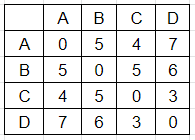
\includegraphics[width=0.3\columnwidth]{mat1.png}
\end{center}
\end{problem}
\begin{center}
\begin{itemize}
		\item Etape 1 :
			\begin{itemize}
			\item On calcule d'abord les valeurs U :
				\[ u_{a} = \frac{5+4+7}{2} = 8 \]
				\[ u_{b} = \frac{5+5+6}{2} = 8 \]
				\[ u_{c} = \frac{4+5+3}{2} = 6 \]
				\[ u_{d} = \frac{7+6+3}{2} = 8 \]
			\item On calcule ensuite les valeurs Q :
				\[ q_{a,b} = 5-8-8 = -11 \]
				\[ q_{a,c} = 4-8-6 = -10 \]
				\[ q_{a,d} = 7-8-8 = -9 \]
				\[ q_{b,c} = 5-8-6 = -9 \]
				\[ q_{b,d} = 5-8-8 = -10 \]
				\[ q_{c,d} = 3-8-6 = -11 \]
			\item On choisit la valeur Q minimale : Ici la valeur Q pour a,b.
			\item On recalcule les distances au nouveau noeud AB :
				\[ d_{ab,c} = \frac{4+5-5}{2} = 2 \]
				\[ d_{ab,d} = \frac{7+6-5}{2} = 4 \]	
			\item On calcule les distances des branches :
				\[ d_{a,ab} = \frac{5}{2} + \frac{(8+8)}{2} = 2.5 \]
				\[ d_{b,ab} = \frac{5}{2} + \frac{(8+8)}{2} = 2.5 \]
			\item Cela nous donne le nouveau tableau :
				\begin{center}
					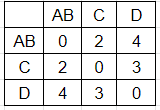
\includegraphics[width=0.27\columnwidth]{mat2.png} 
				\end{center}
			\end{itemize}
		\item Étape 2 :
			\begin{itemize}
			\item On calcule d'abord les valeurs U :
				\[ u_{ab} = \frac{2+4}{1} = 6 \]
				\[ u_{c} = \frac{2+3}{1} = 5 \]
				\[ u_{d} = \frac{4+3}{1} = 7 \]
			\item On calcule ensuite les valeurs Q :
				\[ q_{ab,c} = 2-6-5 = -9 \]
				\[ q_{ab,d} = 4-6-7 = -9 \]
				\[ q_{c,d} = 3-7-5 = -9 \]
			\item On choisit la valeur Q minimale : Ici la valeur Q pour ab,c.
			\item On recalcule les distances au nouveau noeud ABC :
				\[ d_{abc,d} = \frac{3+4-2}{2} = 2.5 \]
			\item On calcule les distances des branches :
				\[ d_{ab,abc} = \frac{2}{2} + \frac{(6-5)}{2} = 0.5 \]
				\[ d_{c,abc} = \frac{2}{2} + \frac{(5-6)}{2} = 1.5 \]
			\item Cela nous donne le nouveau tableau :
				\begin{center}
					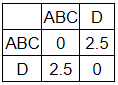
\includegraphics[width=0.25\columnwidth]{mat3.png} 
				\end{center}
			\end{itemize}
		\item On peut maintenant construire l'arbre de phylogénétique :
			\begin{center}
				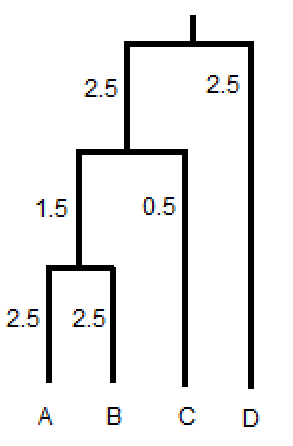
\includegraphics[width=0.4\columnwidth]{arbre.png} 
			\end{center}
	\end{itemize}
	\
\end{center}

%------------------------------------------------

\end{document}
